\chapter{Desenvolvimento do trabalho}

% Apresentar os resultados das fases que transformam
% os requisitos em produtos finais.
% • A estrutura desse capítulo depende do processo de
% desenvolvimento do trabalho.
% • A organização e as seções desse capítulo devem ser
% definidas juntamente com o orientador.

Este capítulo tem como objetivo explicitar quais foram as decisões de projeto que foram tomadas ao longo do desenvolvimento do sistema.

\section{Justificativas das métricas escolhidas}

A escolha das métricas para o desenvolvimento desse projeto foi determinante para avaliar e interpretar resultados com precisão e, como era o objetivo do trabalho, avaliar o perfil de motoristas.

Uma conversa com um funcionário da empresa Porto Seguro foi determinante para ratificar a relevância das métricas definidas. Essa conversa pode ser vista no Apêndice 7.1 deste documento.

\subsection{Gasto do motor a partir do RPM}

Em um motor de combustão interna, o RPM indica a velocidade com que os pistões se movem para cima e para baixo no cilindro. O controle preciso do RPM é essencial para otimizar a eficiência do motor e a entrega de potência, sendo um indicador chave para os motoristas ajustarem suas velocidades de condução.

A figura \ref{fig:rpmxpotencia} mostra que a potência gasta por um motor aumenta quando a rotação dele também ascende\textsuperscript{[28]}. 
 
Dado que a amplitude de tais ondulações (alto RPM) reduz ao longo da vida útil de um pistão, deve-se levar em consideração o efeito do desgaste ao especificar a rugosidade superficial da saia do pistão. Caso contrário, o pistão poderá vir a engripar no cilindro por não ser capaz
de reter óleo em sua superfície \textsuperscript{[40]}.

Durante o funcionamento do motor, a biela fica sujeita a forças de compressão muito elevadas, provenientes da fase de expansão do cilindro e a forças de tração, nas fases de admissão do motor. Sendo assim, as bielas são mais solicitadas nas condições de plena carga e de elevadas rotações do motor\textsuperscript{[40]}.


 \begin{figure}[hp]
    \centering
    
    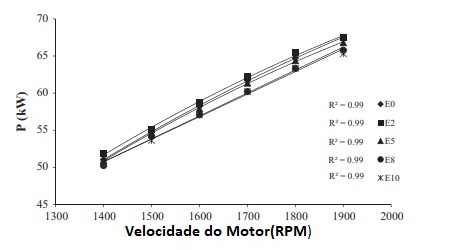
\includegraphics[scale= 1]{figures/rpmxpotencia.jpeg}
    
    \caption{Potência gasta pelo motor em função de sua rotação.}
    
    \label{fig:rpmxpotencia}
\end{figure}

\subsection{Trajetos e rotas perigosas}

A relação entre rotas perigosas, marcadas por assaltos e roubos de carros e o perfil do motorista torna-se um elemento crítico na gestão da segurança. A escolha da rota desempenha um papel significativo na mitigação desses perigos. 

Motoristas que optam por passar frequentemente por áreas consideradas de alto risco podem estar mais suscetíveis a incidentes indesejados. Portanto, compreender o perfil do motorista em relação a essas rotas perigosas é importante para a implementação de estratégias eficazes de prevenção. 

A conscientização dos motoristas sobre áreas de risco pode contribuir para um comportamento mais prudente ao planejar e seguir rotas.

Na cidade de São Paulo, locais como Paulista, Augusta e Sé possuem altos índices de furtos\textsuperscript{[34]}. A figura \ref{fig:mapa_calor_violencia} mostra as áreas com maior índice de assaltos na metrópole.

\begin{figure}[hp]
    \centering
    
    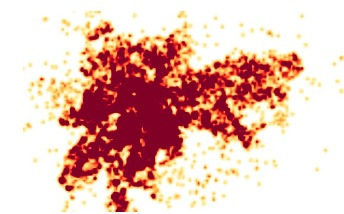
\includegraphics[scale= 1]{figures/mapa_calor_violencia.jpeg}
    
    \caption{Mapa de calor dos incidentes criminais na cidade de São Paulo. Com atenção, é possível ver o contorno da cidade nesta imagem.}
    \label{fig:mapa_calor_violencia}
    
\end{figure}

A figura \ref{fig:mapa_risco_acc_rpm} ilustra alguns dos metadados que podem ser gerados com a análise dos dados obtidos. De forma semelhante, as tabelas \ref{Tb:tab_fracao_acc} e \ref{Tb:tab_fracao_perigo} detalham quanto por cento do tempo o motorista passa acelerando o carro e também a fração de tempo passada em cada região da cidade, respectivamente. Ambas as métricas são subdivididas em três categorias: baixo, médio e alto risco.

\begin{table}[]

    \caption{Exemplo de análise qualitativa da aceleração do carro durante a coleta de dados.}
    \label{Tb:tab_fracao_acc}
    \centering

    \begin{center}
    % \begin{tabular}{lllll}
    % \begin{adjustbox}{width=\textwidth}
        \begin{tabular}{ccc p{6cm} ccc}
            % \rowcolor[HTML]{C0C0C0}
            % \cline[2-3]
            
            \multicolumn{1}{l}{}  & \multicolumn{1}{|l}{
                \textbf{Fração do tempo com cada tipo de aceleração}
            }  \\
            
            % \cellcolor[HTML]{C0C0C0} \textbf{Fração do tempo com cada tipo de aceleração}}  \\

            \hline
            
            \multicolumn{1}{l|}{Aceleração normal}  & \multicolumn{1}{|l}{0,00\%}    \\

            \hline
            
            \multicolumn{1}{l|}{Aceleração média}  & \multicolumn{1}{|l}{55,30\%}    \\

            \hline
            
            \multicolumn{1}{l|}{Aceleração muito alta}  & \multicolumn{1}{|l}{44,70\%}    \\
        \end{tabular}
    % \end{adjustbox}
    \end{center}
\end{table}

% \input{tabelas/tab_fracao_rpm}
\begin{table}[]

    \caption{Exemplo de análise qualitativa de por onde o carro passa durante a coleta de dados.}
    \label{Tb:tab_fracao_perigo}
    \centering

    \begin{center}
    % \begin{tabular}{lllll}
    % \begin{adjustbox}{width=\textwidth}
        \begin{tabular}{ccc p{6cm} ccc}
            % \rowcolor[HTML]{C0C0C0}
            % \cline[2-3]
            
            \multicolumn{1}{l}{}  & \multicolumn{1}{|l}{
                \textbf{Fração do tempo passada em cada tipo de lugar}
            }  \\
            
            % \cellcolor[HTML]{C0C0C0} \textbf{Fração do tempo com cada tipo de aceleração}}  \\

            \hline
            
            \multicolumn{1}{l|}{Baixo risco}  & \multicolumn{1}{|l}{54,55\%}    \\

            \hline
            
            \multicolumn{1}{l|}{Médio risco}  & \multicolumn{1}{|l}{45,45\%}    \\

            \hline
            
            \multicolumn{1}{l|}{Alto risco}  & \multicolumn{1}{|l}{44,70\%}    \\
        \end{tabular}
    % \end{adjustbox}
    \end{center}
\end{table}


% \begin{figure}[hp]
%     \centering
    
%     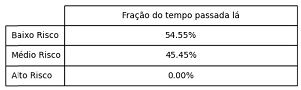
\includegraphics[scale= 1]{figures/tabela_fracao1.jpg}
    
%     \caption{Potência versus velocidade do motor.}
    
    
% \end{figure}

\begin{figure}[hp]
    \centering
    
    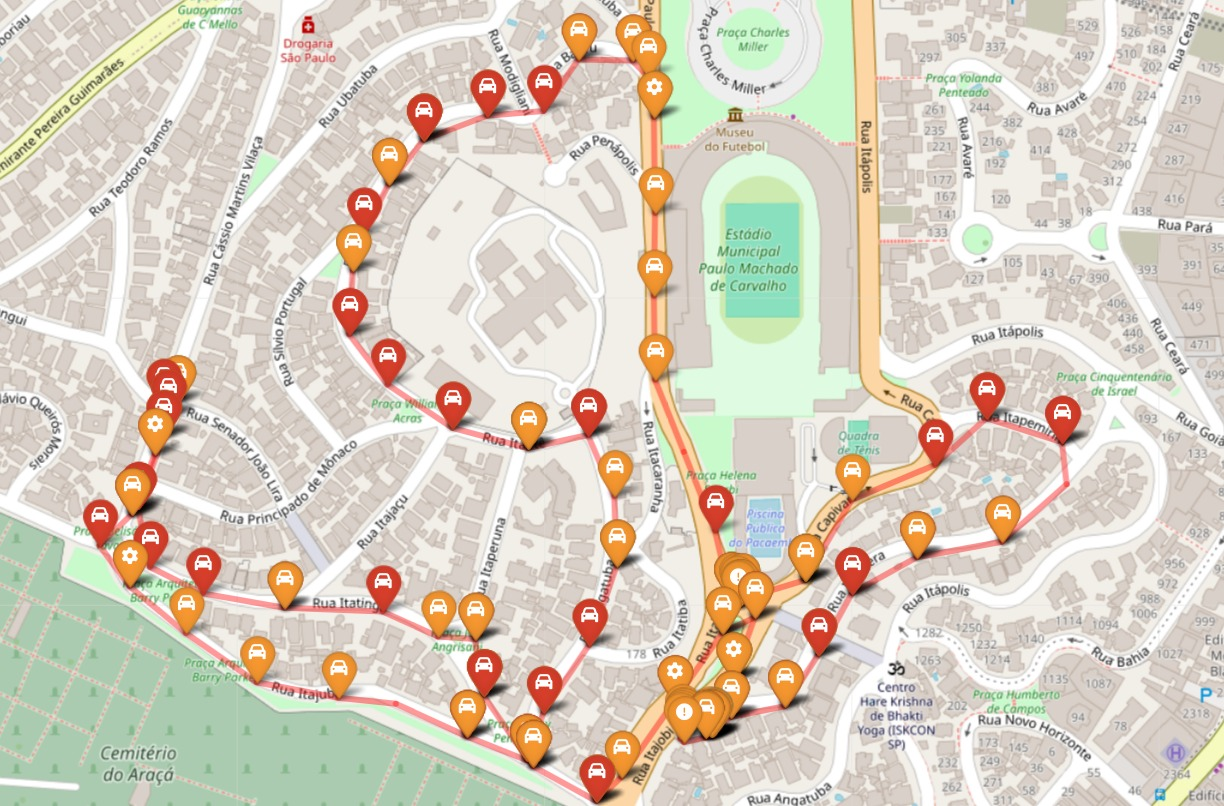
\includegraphics[scale=0.25]{figures/mapa_risco_acc_rpm.jpeg}
    
    \caption{Mapa de risco em acelerações (símbolo de carro) e valores de RPM (símbolo de engrenagem).}
    
    \label{fig:mapa_risco_acc_rpm}
\end{figure}


% \begin{figure}[hp]
%     \centering
    
%     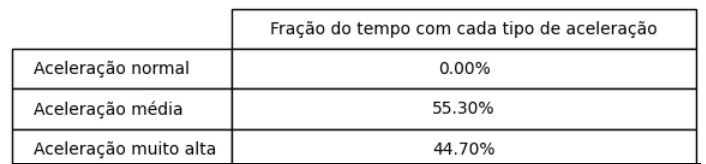
\includegraphics[scale= 0.85]{figures/tabela_2.jpg}
    
%     \caption{Fração da aceleração.}
    
%     \label{fig:tab1}
% \end{figure}

% \begin{figure}[hp]
%     \centering
    
%     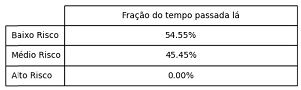
\includegraphics[scale= 0.95]{figures/tabela_fracao1.jpg}
    
%     \caption{Tipo de risco.}
    
%     \label{fig:tab2}
% \end{figure}


A construção dessa figura foi feita graças a uma base de dados encontrada no site Kaggle\textsuperscript{[33]}, conhecido por hospedar \textit{Jupyter Notebooks} analisando certos conjuntos de informações.

Embora a descrição do \textit{dataset} mencione que os dados referem-se só a São Paulo (o que já gera ambiguidade entre cidade e estado), existem lá registros de Curitiba, Rio de Janeiro e Pará também.

Importante mencionar que, devido ao tamanho dessa base de dados, de 12899 linhas, foi preciso pensar-se em como comparar os dados nela contidos com cada um dos registros de GPS fornecidos pelo \textit{app} sem que o desempenho dessa análise fosse comprometido.

Para tal, as coordenadas geográficas da planilha foram indexadas conforme indicado no código-fonte presente no Apêndice 7.5.

Alguns números mágicos (constantes sem derivação algorítmica), que foram utilizados nesse código, levaram em consideração a equivalência entre graus e quilômetros da Terra e as distâncias entre os pontos mais a sul, norte, leste e oeste do Brasil\textsuperscript{[35, 36]}.

A ideia dessa indexação é dividir o mapa em \textit{chunks}, os quais limitam o trabalho computacional a um subconjunto dos dados. Cada \textit{chunk} é um quadrado de lado 500m, o que obriga o programa a olhar alguns blocos adjacentes ao onde está a coordenada cuja segurança quer-se verificar.

% \begin{figure}[hp]
%     \centering
    
%     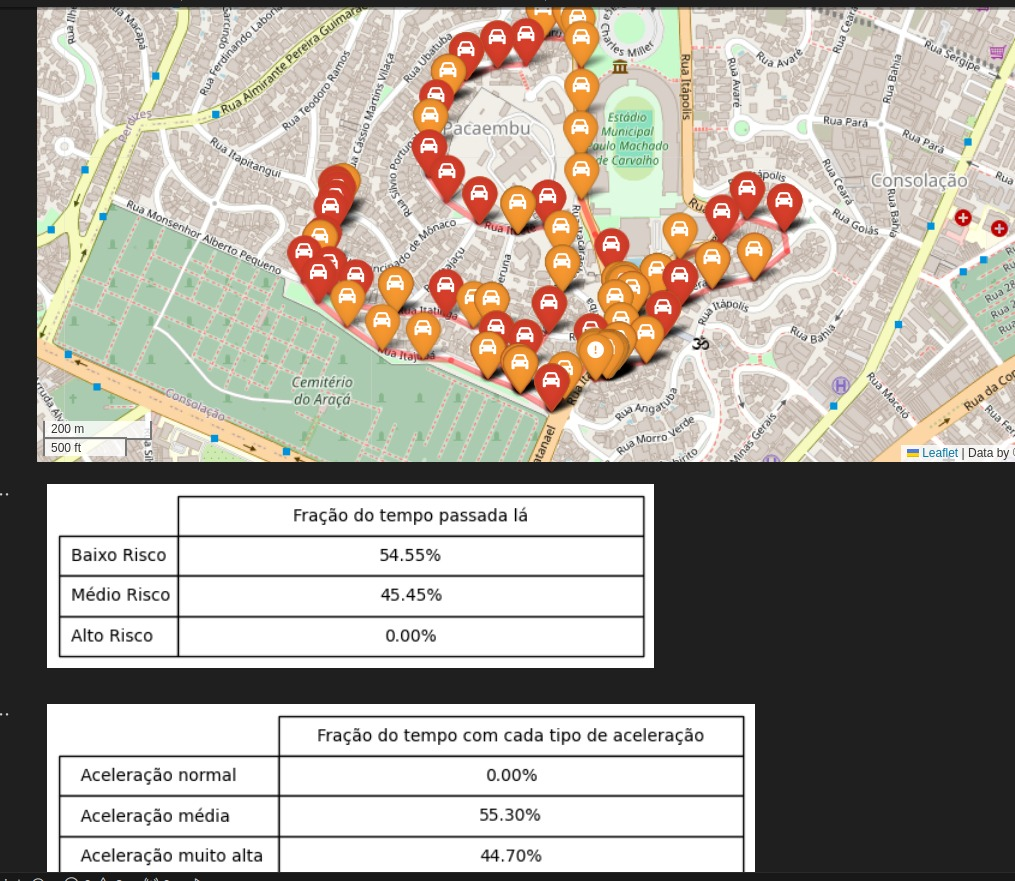
\includegraphics[scale=0.8]{figures/rotas_altorisco.jpeg}
    
%     \caption{}
    
%     \label{fig:rotas_altorisco}
% \end{figure}

 
\section{Tecnologias utilizadas}
O projeto definiu algumas tecnologias de base para serem usadas durante o desenvolvimento de cada fase dele.

    \subsection{Amazon Web Services}

    A escolha da AWS para o projeto é fundamentada em três pilares essenciais: escalabilidade, segurança e viabilidade econômica. 
    
    A capacidade desse serviço de nuvem de se adaptar dinamicamente às demandas do sistema assegura uma infraestrutura flexível, capaz de lidar eficientemente com variações na carga de trabalho. 
    
    Além disso, a reputação consolidada da Amazon em termos de segurança oferece uma base robusta para proteção dos dados e operações. 
    
    Por fim, a viabilidade econômica se destaca, uma vez que a AWS disponibiliza uma variedade de serviços e modelos de precificação que se alinham de maneira eficaz às necessidades do projeto, otimizando custos operacionais.

    É evidente que todas essas vantagens só são concretizadas caso os implementadores do sistema façam uso de toda a funcionalidade da nuvem: projetos monolíticos, ainda que rodados em servidores distribuídos, não exploram a flexibilidade de serviços como a AWS. 

    \subsection{Conexão OBD-II}

    A integração do OBD-II (\textit{On-Board Diagnostics}) neste projeto de sistema de coleta de dados representa um ponto importante na obtenção de dados precisos e abrangentes sobre o desempenho do veículo. 
    
    O OBD-II, um padrão presente em muitos veículos modernos, fornece acesso a uma variedade de parâmetros, como velocidade, rotações por minuto (RPM), temperatura do motor, e códigos de diagnóstico de falhas. 
    
    Ao conectar-se a plataforma de captura de dados ao leitor de OBD-II do veículo, é possível extrair informações em tempo real sobre a condução, condições do motor e possíveis problemas mecânicos.

    Uma plataforma disponibilizada no GitHub que consegue comunicar-se com o veículo através do protocolo OBD-II\textsuperscript{[12]} acelerou o desenvolvimento do projeto, uma vez que o grupo não teve que implementar esse protocolo. 
    
    Esse outro projeto implementa o protocolo OBD-II e também uma interface gráfica básica para mostrar os dados fornecidos pelo carro.

    A figura \ref{fig:obd2_plataforma} mostra a tela principal do \textit{app}, onde é possível ver alguns dos dados gerados durante o dirigir do usuário.

    
\begin{figure}[hp]
    \centering
    
    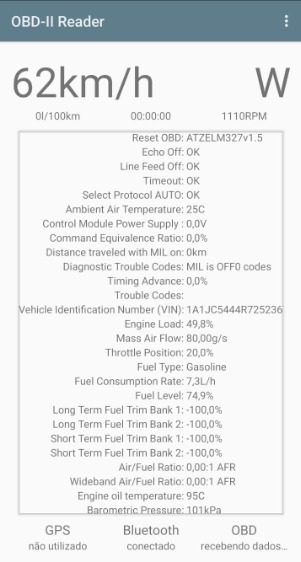
\includegraphics[scale=0.5]{figures/obd2.jpeg}
    
    \caption{Interface inicial do \textit{app} que se comunica com a porta OBD-II\textsuperscript{[12]}.}
    
    \label{fig:obd2_plataforma}
\end{figure}

    \subsection{Simulador de OBD-II}

    A ausência de um carro físico no início do projeto foi contornada por meio da utilização de um simulador de OBD. Esse dispositivo desempenhou um papel crucial como um substituto temporário do automóvel, permitindo que o trabalho continuasse normalmente. 
    
    Em vez de depender de um veículo real, a equipe conseguiu controlar e reproduzir dados e comportamentos típicos de um carro a partir do programa de controle do simulador\textsuperscript{[21]}.

    Além disso, o uso desse dispositivo proporcionou um ambiente controlado para a validação do \textit{software} em diferentes cenários, contribuindo para a eficiência e progresso do projeto enquanto não se podia realizar testes práticos.
    
    \subsection{Android Studio e Java} 
    A utilização da IDE Android Studio neste projeto de sistema de coleta de dados desempenha um papel central no desenvolvimento do aplicativo móvel já mencionado. 
    
    O Android Studio, sendo a principal ferramenta de desenvolvimento para aplicativos Android, oferece um ambiente integrado e robusto que simplifica a criação, os testes e a depuração do \textit{software}. 
    
    A plataforma fornece recursos avançados de \textit{design} de interface do usuário, facilitando a criação de aplicativos intuitivos e visualmente atraentes para os usuários finais. 
    
    A integração perfeita com o Android SDK (\textit{Software Development Kit}) permite o acesso às APIs e recursos específicos do sistema operacional Android, garantindo, através de interfaces do sistema operacional, o uso de \textit{hardwares} de propósito específico, como o que faz a comunicação Bluetooth. 
    
    Além disso, as ferramentas de emulação e depuração incorporadas no Android Studio simplificam o processo de teste em diferentes dispositivos, contribuindo para a criação de aplicativos estáveis e adaptáveis.

    Nenhuma tecnologia multiplataforma (React Native ou Flutter, por exemplo) ou específica de dispositivos iOS (Swift ou Objective C, por exemplo) foi escolhida, pois o intuito do projeto era ser compatível com os celulares dos membros do grupo e devido à familiaridade com a linguagem Java, usada para esse tipo de desenvolvimento.

    O aplicativo em si originalmente foi desenvolvido para a API de versão 22 do Android. Condição que foi alterada para comportar funcionalidades que foram adicionadas ao sistema operacional desde 2013. A versão atual de compilação (versão do SDK) é a 33.

    O desenvolvimento do aplicativo Android envolveu várias etapas, sendo o primeiro passo a modificação apropriada do arquivo \textit{build.gradle}. Este processo, no entanto, consumiu considerável tempo devido à falta de experiência dos membros do grupo. 
    
    Após a configuração inicial, a equipe se dedicou a identificar onde os parâmetros do OBD estavam disponíveis no código-fonte. Esta fase de investigação foi crucial para possibilitar o subsequente envio desses dados para a nuvem.

    No entanto, as dificuldades técnicas foram tão significativas que inicialmente não foi possível realizar o envio de dados para a nuvem. 
    
    Diante desse impasse, uma exceção teve que ser aberta no projeto, resultando na geração de arquivos \textit{.txt} locais no \textit{smartphone} em que o aplicativo estivesse rodando. 
    
    Essa solução permitiu que o trabalho de análise dos dados começasse, já que a produção de informações já estava funcional naquele momento.
    
    Posteriormente, a equipe conseguiu superar os obstáculos e implementou com sucesso o envio de dados para a nuvem, empregando a biblioteca Volley do Android. Essa abordagem proporcionou uma resolução eficaz para a integração com serviços de armazenamento na nuvem, consolidando a funcionalidade do \textit{app}. 

     \begin{figure}[hp]
    \centering
    
    
\includegraphics[scale=0.4]{figures/logo_android.png}
    
    \caption{Logo do Android Studio.}
    
\end{figure}
    
    \subsection{Banco de dados} 
    A integração do MySQL e do AWS RDS (Relational Database Service) em um projeto de sistema de compilação de dados de veículos é uma estratégia robusta para o gerenciamento eficiente e escalável dos dados do sistema. 
    
    O MySQL, um sistema de gerenciamento de banco de dados relacional de código aberto, proporciona uma estrutura confiável para armazenar e organizar informações como histórico de rotas e dados do OBD-II. 
     
     Ao escolher o AWS RDS como a plataforma de hospedagem para o MySQL, ganha-se os benefícios adicionais de escalabilidade automática, alta disponibilidade e segurança avançada oferecidos pela infraestrutura em nuvem da Amazon. A integração dessas tecnologias permite o acesso eficiente aos dados, consultas rápidas e uma gestão simplificada do banco de dados. 
     
     Além disso, o AWS RDS lida com tarefas operacionais, como \textit{backup} automático e manutenção. 
     
     Essa combinação proporciona uma base sólida para o armazenamento e recuperação de dados, promovendo a confiabilidade e eficácia do sistema.

     A estrutura definida para as tabelas do banco de dados foi:


    \begin{itemize}
         \item{\textbf{tcc-schema} (esquema do banco de dados onde se encontram as tabelas)}
         
        \begin{itemize}
             \item{\textbf{info:} Armazena as informações coletadas através da porta OBD} 
        
             \item{\textbf{acceleration:} Contém dados dos acelerômetros do celular do usuário} 
             
             \item{\textbf{location:} Guarda latitude e longitude obtidas por GPS pelo celular}   
        \end{itemize}  
    \end{itemize}

     A especificação exata das colunas de cada tabela pode ser encontrada no Apêndice 7.2.

    \begin{figure}[hp]
        \centering
        
        
\includegraphics[scale=0.4]{figures/logo_Mysql.jpg}
        
        \caption{Logo do Mysql.}
        
    \end{figure}

    Importante mencionar que o tamanho do banco de dados foi limitado a 20GiB, visando impedir que o serviço da AWS cobrasse qualquer valor monetário dos membros do grupo.
    
    O \textit{Free Tier} é um conjunto de limites de execução e armazenamento em nuvem definido para projetos-teste de contas novas na plataforma (com menos de 1 ano de existência\textsuperscript{[40]}). A forma de zerar os gastos com esse projeto é não exceder a fronteira dessas cortesias.

    
    \subsection{\textit{Python}} 

    A versão do Python usada para todos os arquivos \textit{.py} do projeto foi a 3.12.0.

    É importante mencionar que junto a cada módulo feito em Python neste projeto, as dependências necessárias para rodá-los foram escritas em arquivos \textit{requirements.txt}, como pode ser visto nos repositórios outrora mencionados.

%     As seguir um exemplo desse arquivo:

% \begin{python}
% ipykernel
% numpy
% pandas
% matplotlib
% folium
% geopy
% pyproj
% scipy
% plotly-express
% nbformat
% \end{python}

    Para poder-se executar os \textit{Jupyter Notebooks} desenvolvidos, é preciso desencadear os seguintes comandos em um terminal (em sistema operacional \textit{Linux}):

\begin{python}
python3 -m venv .venv
source .venv/bin/activate
python3 -m pip install requirements.txt
\end{python}
    

% \subsubsection{Folium}
     
%      A junção do Python e do Folium em um projeto de sistema de coleta de dados oferece uma poderosa combinação para a visualização interativa e geoespacial dos dados. 
     
%      O Folium é uma biblioteca que simplifica a criação de mapas interativos baseados na \textit{web}. Integrar o Folium ao projeto permite que os desenvolvedores gerem mapas dinâmicos que destacam informações específicas relacionadas ao rastreamento de veículos.

%     % Essa integração Python-Folium é particularmente útil para análises geoespaciais em sistemas de rastreamento de veículos, proporcionando uma representação geográfica e visualmente intuitiva dos dados de telemetria. 
    
%     % A flexibilidade do Python permite a personalização dos mapas e a incorporação de recursos adicionais conforme as necessidades específicas do projeto, contribuindo para uma interface de usuário mais informativa e envolvente.



% interface com usuario, banco de dados, conexão obd2

    % \subsubsection{Flask}

    % A seleção da biblioteca Flask para o projeto ocorreu devido à familiaridade com a linguagem Python, tornando o desenvolvimento mais acessível. Adicionalmente, a escolha se fundamentou na capacidade do Flask em facilitar a implementação eficiente de uma API, atendendo à necessidade do aplicativo de enviar e receber dados de maneira eficaz. O código python da API em Flask foi hospedado em um Lambda da AWS para facilitar o seu uso pelo APP posteriormente.


\section{Projeto e implementação}
% Esta seção descreverá as decisões feitas durante o trabalho.

% \subsection{Folium}
   

    \subsection{Análise de Dados - RideParser}\label{rideparser}

    A função da classe RideParser é analisar dados dos trajetos feitos pelos motoristas. 
    
    Alguns filtros são recebidos pelo construtor dessa classe, para personalizar a geração de gráficos. Esses parâmetros são usados para restringir o que vem do banco de dados a uma certa janela de tempo e ao usuário que solicita aquela informação.
    
    % Já o módulo 
    % ''os'' fornece funcionalidades relacionadas ao sistema operacional, permitindo que você interaja com o ambiente do sistema, como manipular diretórios, arquivos, obter informações sobre o sistema, manipular variáveis de ambiente, entre outras tarefas relacionadas ao sistema operacional.
    Dentro desse mesmo arquivo, algumas bibliotecas típicas de ciência de dados foram utilizadas para manipular os gráficos mencionados. Foram elas: pandas, matplotlib, numpy e scipy.
    
    A figura \ref{fig:rota_uah_driveset} mostra o video e o gráfico da aceleração de um carro. Os dados foram pegos de um repositório chamado UAH-Driveset\textsuperscript{[42]}, disponível na \textit{internet}.
    
    \begin{figure}[hp]
        \centering
        
        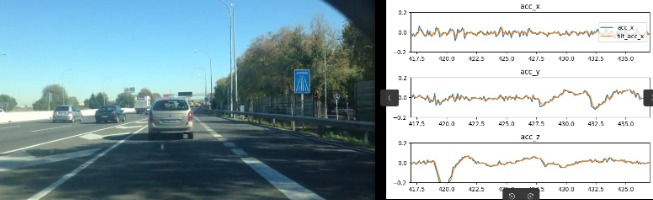
\includegraphics[scale=0.6]{figures/rota_uah_driveset.jpg}
        
        \caption{Rota de uma viagem de um dos integrantes do grupo.}
        \label{fig:rota_uah_driveset}
    \end{figure}

    \subsection{API Rest - Flask}
    A implementação da API centraliza-se em uma arquitetura Python utilizando a biblioteca Flask, proporcionando uma estrutura ágil e eficiente para a comunicação com a base de dados MySQL, hospedada em um serviço de RDS na AWS. A escolha da linguagem Python e do framework Flask foi motivada pela sua simplicidade e flexibilidade, permitindo a rápida construção dos \textit{endpoints} responsáveis pela interação entre o aplicativo e a base de dados.

    A lógica da API foi encapsulada em funções específicas, acionadas por meio de requisições POST. O corpo do JSON enviado nessas requisições determina a ação a ser executada, que pode ser uma entre seis operações distintas. Três destas operações referem-se a consultas (GET) e três a modificações (POST), cada uma vinculada a uma das três tabelas da base de dados.

    Para facilitar a utilização da API pelo \textit{app}, o código Python foi integrado ao ambiente \textit{serverless} da AWS Lambda. 
    
    Essa escolha estratégica permite que as funções sejam invocadas sob demanda, proporcionando uma resposta ágil às requisições do aplicativo Android, que, por sua vez, está sendo desenvolvido no ambiente Java do Android Studio. 
    
    A combinação dessas tecnologias promove uma arquitetura eficiente para gerenciar a comunicação entre o aplicativo e a infraestrutura de banco de dados na nuvem.

    \subsection{Folium}

\begin{figure}[hp]
    \centering
    
    
\includegraphics[scale=0.1]{figures/python_folium.jpg}
    
    \caption{Logos do Python e do Folium.}
\end{figure}

 Para criar os mapas do aplicativo, foi utilizado o \textit{framework} Folium. Essa biblioteca é uma poderosa ferramenta para manipular e visualizar dados geoespaciais usando Python. 
    
    Com o Folium, é possível criar mapas interativos personalizados e incorporar dados neles de várias maneiras. Para manipular dados usando essa ferramenta, pode-se começar importando a biblioteca e criando um objeto \textit{Map}, que representa o mapa. 
    
    Em seguida, pode-se adicionar camadas, como marcadores, polígonos e \textit{popups}, para exibir dados de forma intuitiva no mapa. 
    
    % O Folium permite a integração de dados geoespaciais em diferentes formatos, como GeoJSON, tornando-o uma ferramenta flexível para análise e visualização de dados geoespaciais em Python. 
    
    A figura 
    \ref{fig:python_libs} mostra as bibliotecas utilizadas para desenvolver os mapas do projeto.
    
    \begin{figure}[hp]
        \centering
        
        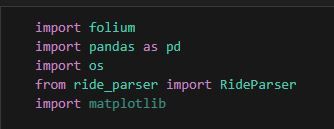
\includegraphics[scale=0.8]{figures/bibliotecas.jpg}
        
        \caption{Bibliotecas utilizadas para gerar o mapa da rota do usuário.}
        
        \label{fig:python_libs}
    \end{figure}
    
            % \begin{center}
            %  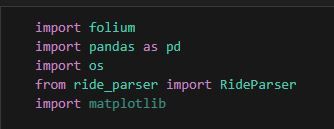
\includegraphics[scale=0.8]{figures/bibliotecas.jpg}
            %  
            %  \end{center}
            
    Para traçar uma trajetória no mapa usando a biblioteca Folium em Python, é necessária uma lista de pontos de latitude e longitude que representam a trajetória. 
    
    A partir dos pontos colhidos pelo GPS do celular, cria-se um mapa da trajetória descrita. A demonstração de uma trajetória recriada em um mapa usando Folium pode ser vista na figura \ref{fig:car_route_1}.
    
    \begin{figure}[hp]
        \centering
        
        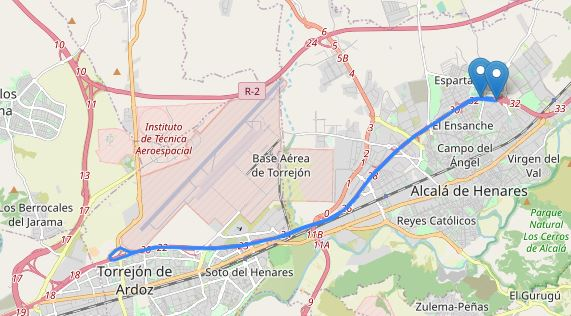
\includegraphics[scale=0.8]{figures/rota_1.jpg}
        
        \caption{Rota de uma das viagens fornecidas pelo \textit{UAH Driveset}.}
        
        \label{fig:car_route_1}
    \end{figure}
    
    O grupo procurou correlacionar eventos de anormalidade nos dados de aceleração do UAH Drivest observando o comportamento da curva dessa grandeza física no tempo e comparando com os eventos do vídeo que acompanhava cada uma das pastas disponibilizadas, mas nenhuma funcionalidade foi adicionada à análise dos dados devido a essa escolha.
    


    \subsection{Criação de relatório de direção em PDF}
    
    A geração de \textit{insights} visuais e análise métrica a partir dos dados armazenados na base MySQL é um componente essencial do projeto. 
    
    A decisão de fazer isso através da geração de um PDF para o motorista baseou-se na clareza e simplicidade desse formato de arquivo. 
    
    Essa escolha é respaldada também pela facilidade de implementação, disponibilizada pelas bibliotecas \textit{Matplotlib} e \textit{Reportlab}, que permitem a criação de PDFs formatados contendo os gráficos com as métricas geradas.
    
    Um segundo AWS Lambda desempenha papel central nesse processo, funcionando como uma ponte entre a base de dados e as ferramentas de visualização. 
    
    Ao ser acionado, o Lambda gerador de PDF realiza uma chamada ao outro Lambda, que extrai as informações relevantes da base de dados MySQL referentes ao usuário, para realizar a análise.

    Utilizando a biblioteca \textit{Matplotlib} em Python, a função Lambda então emprega métodos da classe RideParser, mencionada na seção \ref{rideparser}, para criar um relatório do motorista, com gráficos e métricas relevantes referentes a sua condução. Isso proporciona aos usuários uma compreensão mais aprofundada das métricas associadas às suas atividades.
    
    Para proporcionar aos usuários uma maneira acessível de interagir com esses \textit{insights}, um botão "gerar PDF" foi incorporado no aplicativo. Este botão aciona o segundo Lambda, que compila os gráficos e métricas gerados em um arquivo PDF. 
    
    A utilização da biblioteca \textit{smtplib} facilita o envio desse PDF diretamente para o usuário via \textit{email}. Essa solução integrada oferece uma experiência completa aos usuários, permitindo-lhes não apenas visualizar, mas também compartilhar os resultados de suas análises de maneira simples.    

    \subsection{Autenticação com \textit{Firebase}}

    A  escolha do \textit{Firebase} para a identificação única do usuário no sistema decorre da capacidade da plataforma em oferecer eficiência e segurança nesse processo, diminuindo-se a carga de responsabilidade do sistema em armazenar informações sensíveis de cada pessoa. 
    
    Essa decisão é fundamentada pela praticidade proporcionada pela integração do \textit{Firebase} com aplicativos \textit{Android} e páginas web\textsuperscript{[29]}, simplificando a implementação de autenticação e gestão de usuários, assegurando uma identificação singular e segura no âmbito do sistema em questão.

    \subsection{Dependências do Gradlle}

    Em um primeiro instante o \textit{app} android-obd-reader não rodava na IDE Android studio. 
    
    Para que fosse possível compilar o projeto, alterações no arquivo \textbf{gradle/wrapper/gradle-wrapper.properties} foram necessárias. 
    
    Atualizar as dependências do Gradle  é muitas vezes pré-condição para garantir que um aplicativo possa se beneficiar das correções de \textit{bugs}, melhorias de desempenho e novos recursos fornecidos pelas versões mais recentes das bibliotecas que estão sendo utilizadas. Este ponto na história do repositório mostra as alterações que foram necessárias: \url{https://github.com/APF2000/android-obd-reader-pires/commit/def70ed262b1fad28cc9e2b98a48af45cfac5695}.

    \subsection{Proteção dos dados}
    
    Na Lei Geral de Proteção de Dados (Lei n. 13.709/18-LGPD), parte-se da ideia de que todo dado pessoal tem importância e valor. 
    
    Por essa razão, este projeto levou em consideração o conceito amplo de dado pessoal, assim como estabelecido no Regulamento Europeu \textsuperscript{[30]} (\textit{GDPR-General Data Protection  Regulation}). 
    
    Quando se trata de um aplicativo projetado para analisar o perfil do motorista de carros, a LGPD impõe uma série de responsabilidades e requisitos ao desenvolvedor e operador do aplicativo. 
    
    É necessário obter o consentimento  do usuário antes de coletar e processar quaisquer dados pessoais relacionados ao seu perfil de condução.
    
    Além disso, a LGPD exige que medidas de segurança apropriadas sejam implementadas para proteger esses dados contra acessos não autorizados e vazamentos. Os usuários têm o direito de acessar, corrigir e excluir suas informações pessoais, e o aplicativo deve fornecer meios para que esses direitos sejam exercidos.

    Por simplicidade, este trabalho não cumpriu essas regras, mas o grupo tem ciência das vulnerabilidades e dos pontos de melhoria nesse aspecto.


% Using \texttt{biblatex} you can display a bibliography divided into sections, depending on citation type. 
% Let's cite! Einstein's journal paper \cite{einstein} and Dirac's book \cite{dirac} are physics-related items. 
% Next, \textit{The \LaTeX\ Companion} book \cite{latexcompanion}, Donald Knuth's website \cite{knuthwebsite}, \textit{The Comprehensive Tex Archive Network} (CTAN) \cite{ctan} are \LaTeX-related items; but the others, Donald Knuth's items, \cite{knuth-fa,knuth-acp} are dedicated to programming. 




\section{Testes e avaliação}
% descrever o plano de testes do sistema: testes de software, modulo, integração e validação
Alguns testes foram definidos para a ratificação das funcionalidades do sistema:

\begin{itemize}
    \item \textbf{Conferir conexão OBD-II:} 
    
    \begin{itemize}
        \item Conectar o dispositivo de leitura na entrada do carro
        \item Ligar a comunicação \textit{bluetooth} do celular
        \item Parear os dois dispositivos
        \item Digitar a senha 1234, padrão dos dispositivos de leitura OBD
        \item Ligar a coleta de dados através do aplicativo
        \item A tela deve sinalizar que o protocolo está sendo feito da forma correta
    \end{itemize}
    
    \item \textbf{Teste de continuidade de transferência de dados:} 
    \begin{itemize}
        \item Fazer conexão com o OBD conforme descrito no teste anterior
        \item Andar com o carro por alguns minutos com a tela do celular desbloqueada (de preferência mudar o \textit{timeout} da tela nas configurações do celular)
        \item Atestar que nenhum dado foi perdido por falta de conexão (pode ser visto por descontinuidade dos gráficos)
    \end{itemize}
    
    \item \textbf{Equivalência de envio e recepção de dados:}
    \begin{itemize}
        \item Comparar o \textit{log} de envio de dados do aplicativo de interface com a porta OBD-II com o \textit{log} de salvamento do banco de dados hospedado na nuvem
        \item A quantidade de dados, os \textit{timestamps} deles e seus conteúdos devem ser idênticos
    \end{itemize}
    
    \item \textbf{Testes de segurança:} 
    \begin{itemize}
        \item Ratificar que não é possível ter acesso aos dados de um certo usuário sem ter as informações de \textit{login}
        \item Verificar o certificado SSL do remetente e só aceitar a mensagem se a informação condisser com as credenciais armazenadas daquele usuário
    \end{itemize}
    
    \item \textbf{Geração de dados \textit{outliers}:}
    \begin{itemize}
        \item Verificar se o sistema descarta corretamente as informações que fogem totalmente do padrão esperado ou se consegue pelo menos esconder isso do usuário
        \item Os PDFs gerados com o sistema devem sofrer um processo de análise de plausibilidade, o que deve averiguar que a análise automática está sendo feita corretamente
    \end{itemize}
    
\end{itemize}


\subsection{Fluxo de uso do sistema}

    \begin{itemize}
    \item \textbf{Autenticação com o Google:}
    O aplicativo no celular deve ser iniciado para realizar a autenticação com as credenciais do Google, assegurando uma identificação segura do usuário.

    \item \textbf{Conexão com o OBD:}
    A conexão entre o celular e o OBD deve ser estabelecida, garantindo que o leitor esteja corretamente emparelhado para iniciar a comunicação.

    \item \textbf{Início da Coleta de Dados:}
    A coleta de dados deve ser ativada por meio do aplicativo.

    \item \textbf{Condução do Veículo:}
    O veículo deve ser conduzido normalmente, permitindo que o aplicativo faça a coleta de dados em tempo real.

    \item \textbf{Posicionamento Fixo do Celular:}
    O celular deve ser fixado em uma posição estável dentro do veículo usando um suporte apropriado. Isso garantirá que os dados de aceleração sejam confiáveis, o que evitará qualquer tipo de interferência na análise posterior da direção.
\end{itemize}


\subsection{Carros utilizados para teste}

    A escolha dos carros onde o leitor de OBD seria conectado foi feita a partir dos veículos de familiares.

    Os modelos em que o sistema foi testado, foram em maioria para analisar quais parâmetros de OBD haviam sido implementados em todos eles.

    Os carros usados foram:

    \begin{itemize}
        \item Hyundai Ix35 - 2012
        \item Mercedes C200 CGI - 2014
        \item Ford Xsport - 2008
    \end{itemize}

    
    O modelo Ix35 foi a principal fonte de dados do projeto, pois praticamente todos os testes feitos para a nova base de dados foram feitos com ele.

    \subsection{Aparelhos \textit{smartphone}}

    O aplicativo foi rodado em dois modelos diferentes de celular:
    \begin{itemize}
        \item Samsung Galaxy A71
        \item Samsung Galaxy S9
        \item Samsung Galaxy S22
        \item Motorola Moto G
    \end{itemize}

\subsection{Definição de dados relevantes para o perfilamento}

    Os parâmetros identificados em comum em todos os carros testados foram: \textit{AIR-FUEL-RATIO, AIR-INTAKE-TEMP, AMBIENT-AIR-TEMP, BAROMETRIC-PRESSURE, CONTROL-MODULE-VOLTAGE, DISTANCE-TRAVELED-MIL-ON, DTC-NUMBER, ENGINE-COOLANT-TEMP, ENGINE-LOAD, ENGINE-OIL-TEMP, ENGINE-RPM, ENGINE-RUNTIME, EQUIV-RATIO, Echo Off, FUEL-CONSUMPTION-RATE, FUEL-LEVEL, FUEL-PRESSURE, FUEL-RAIL-PRESSURE, FUEL-TYPE, INTAKE-MANIFOLD-PRESSURE, Line Feed Off, Long Term Fuel Trim Bank 1, Long Term Fuel Trim Bank 2, MAF, Reset OBD, SPEED, Select Protocol AUTO, Short Term Fuel Trim Bank 1, Short Term Fuel Trim Bank 2, THROTTLE-POS, TIMING-ADVANCE, TROUBLE-CODES, Timeout, VIN, WIDEBAND-AIR-FUEL-RATIO}.

    No entanto, muitas dentre essas informações ou apresentavam o valor \textit{NODATA}, que significa que estavam sendo amostrados pelo OBD, mas não continham dados válidos, ou apresentavam dados constantes, os quais independem da direção do motorista.

    Os \textbf{parâmetros descartados} foram \textit{CONTROL-MODULE-VOLTAGE, DISTANCE-TRAVELED-MIL-ON, DTC-NUMBER, Echo Off, ENGINE-OIL-TEMP, FUEL-CONSUMPTION-RATE, FUEL-LEVEL, FUEL-PRESSURE, FUEL-RAIL-PRESSURE, FUEL-TYPE, Line Feed Off, Long Term Fuel Trim Bank 2, MAF, Reset OBD, Select Protocol AUTO, Short Term Fuel Trim Bank 2, Timeout, TROUBLE-CODES, VIN, WIDEBAND-AIR-FUEL-RATIO}.
    
    Os \textbf{parâmetros considerados} para uso foram \textit{AIR-FUEL-RATIO, AIR-INTAKE-TEMP, AMBIENT-AIR-TEMP, BAROMETRIC-PRESSURE, ENGINE-COOLANT-TEMP, ENGINE-LOAD, ENGINE-RPM, ENGINE-RUNTIME, EQUIV-RATIO, INTAKE-MANIFOLD-PRESSURE, Long Term Fuel Trim Bank 1, Short Term Fuel Trim Bank 1, SPEED, THROTTLE-POS, TIMING-ADVANCE}.
    
    Entre os dados candidatos para serem usados no projeto, apenas os que foram \textbf{citados em artigos científicos} como determinantes para o acontecimento de acidentes e a deterioração do carro foram de fato levados em consideração: \textit{ENGINE-RPM}\textsuperscript{[28]}, \textit{SPEED}\textsuperscript{[32]}

            %     \item CONTROL-MODULE-VOLTAGE
            % \item DISTANCE-TRAVELED-MIL-ON
            % \item DTC-NUMBER
            % \item Echo Off
            % \item ENGINE-OIL-TEMP
            % \item FUEL-CONSUMPTION-RATE
            % \item FUEL-LEVEL
            % \item FUEL-PRESSURE
            % \item FUEL-RAIL-PRESSURE
            % \item FUEL-TYPE
            % \item Line Feed Off
            % \item Long Term Fuel Trim Bank 2
            % \item MAF
            % \item Reset OBD
            % \item Select Protocol AUTO
            % \item Short Term Fuel Trim Bank 2
            % \item Timeout
            % \item TROUBLE-CODES
            % \item VIN
            % \item WIDEBAND-AIR-FUEL-RATIO

            % \item AIR-FUEL-RATIO
            % \item AIR-INTAKE-TEMP
            % \item AMBIENT-AIR-TEMP
            % \item BAROMETRIC-PRESSURE
            % \item ENGINE-COOLANT-TEMP
            % \item ENGINE-LOAD
            % \item ENGINE-RPM
            % \item ENGINE-RUNTIME
            % \item EQUIV-RATIO
            % \item INTAKE-MANIFOLD-PRESSURE
            % \item Long Term Fuel Trim Bank 1
            % \item Short Term Fuel Trim Bank 1
            % \item SPEED
            % \item THROTTLE-POS
            % \item TIMING-ADVANCE


    % \begin{itemize}
    %     \item AIR-FUEL-RATIO
    %     \item AIR-INTAKE-TEMP
    %     \item AMBIENT-AIR-TEMP
    %     \item BAROMETRIC-PRESSURE
    %     \item CONTROL-MODULE-VOLTAGE
    %     \item DISTANCE-TRAVELED-MIL-ON
    %     \item DTC-NUMBER
    %     \item ENGINE-COOLANT-TEMP
    %     \item ENGINE-LOAD
    %     \item ENGINE-OIL-TEMP
    %     \item ENGINE-RPM
    %     \item ENGINE-RUNTIME
    %     \item EQUIV-RATIO
    %     \item Echo Off
    %     \item FUEL-CONSUMPTION-RATE
    %     \item FUEL-LEVEL
    %     \item FUEL-PRESSURE
    %     \item FUEL-RAIL-PRESSURE
    %     \item FUEL-TYPE
    %     \item INTAKE-MANIFOLD-PRESSURE
    %     \item Line Feed Off
    %     \item Long Term Fuel Trim Bank 1
    %     \item Long Term Fuel Trim Bank 2
    %     \item MAF
    %     \item Reset OBD
    %     \item SPEED
    %     \item Select Protocol AUTO
    %     \item Short Term Fuel Trim Bank 1
    %     \item Short Term Fuel Trim Bank 2
    %     \item THROTTLE-POS
    %     \item TIMING-ADVANCE
    %     \item TROUBLE-CODES
    %     \item Timeout
    %     \item VIN
    %     \item WIDEBAND-AIR-FUEL-RATIO
    % \end{itemize}